% \begin{name}
% 	{GV biên soạn: Hồ Ngọc Nhất Linh\\ GV phản biện: }
% 	{TOÁN 10-KNTT-CS}
% \end{name}
%----------------NỘI DUNG BIÊN SOẠN
% \setcounter{chapter}{1}
\chap{BẤT PHƯƠNG TRÌNH VÀ HỆ BẤT PHƯƠNG TRÌNH BẬC NHẤT HAI ẨN}
\def\tenchude{BẤT PHƯƠNG TRÌNH BẬC NHẤT HAI ẨN}

\setcounter{section}{2}
\section{Bất phương trình bậc nhất hai ẩn}
%-------------------------------------------
\subsection{KIẾN THỨC TRỌNG TÂM}
\subsubsection{Bất phương trình bậc nhất hai ẩn}
\begin{khung4}{}
Bất phương trình bậc nhất hai ẩn $x$, $y$ có dạng tổng quát là
$$
ax+by+c\leq 0.\quad (*)$$
$$(\text{hoặc }ax+by+c<0, \text{ hoặc } ax+by+c\geq 0, \text{ hoặc }ax+by+c>0).
$$
Trong đó $a$, $b$, $c$ là những số thực và $a^2+b^2 > 0$.\\
Cặp số $\left(x_0;y_0\right)$ là nghiệm của $(*)\Leftrightarrow ax_0+by_0+c\leq 0$.
\end{khung4}
\subsubsection{Miền nghiệm của bất phương trình bậc nhất hai ẩn}

\begin{khung4}{}
	Trên mặt phẳng $Oxy$, đường thẳng $d\colon ax+by=c$ chia mặt phẳng thành hai nửa mặt phẳng. Một trong hai nửa mặt phẳng (không kể $d$) là \textit{miền nghiệm} của bất phương trình $ax+by<c$, nửa mặt phẳng còn lại (không kể $d$) là \textit{miền nghiệm} của bất phương trình $ax+by>c$.
\end{khung4}
\begin{khung4}{}
	Cho cặp số $\left(x_0;y_0\right)$ là \textbf{nghiệ}m của bất phương trình $ax_0+by_0+c < 0$. Khi đó điểm $M(x_0;y_0)$ \textbf{nằm trong miền nghiệm} của bất phương trình $ax_0+by_0+c < 0$.
\end{khung4}
\subsubsection{Quy tắc biểu diễn miền nghiệm của bất phương trình}
\begin{khung4}{}
	Biểu diễn miền nghiệm của bất phương trình bậc nhất hai ẩn $ax+by+c\geq 0$.\quad $(*)$\\
\textbf{Bước 1:} Vẽ đường thẳng $\Delta\colon ax+by+c=0$.\\
\textbf{Bước 2:} Lấy một điểm $M_0\left(x_0;y_0\right)$ không thuộc $\Delta$ (thường lấy gốc tọa độ $O$).\\
\textbf{Bước 3:} Tính $ax_0+by_0+c$ và so sánh với $0$.\\
\textbf{Bước 4:} Kết luận
	\begin{itemize}
		\item Nếu $ax_0+by_0+c<0$ thì nửa mặt phẳng bờ $\Delta$ chứa $M_0$ là miền nghiệm của $(*)$.
		\item Nếu $ax_0+by_0+c>0$ thì nửa mặt phẳng bờ $\Delta$ không chứa $M_0$ là miền nghiệm của $(*)$.
	\end{itemize}
\begin{note}
	Miền nghiệm của $(*)$ bỏ đi đường thẳng $\Delta$ là miền nghiệm của bất phương trình $ax+by+c<0$.
\end{note}
\end{khung4}
\subsection{PHÂN LOẠI VÀ PHƯƠNG PHÁP GIẢI TOÁN}
\begin{dang}{Kiểm tra nghiệm của bất phương trình bậc nhất hai ẩn}
	{\it Phương pháp:}\\
	Cho cặp số $\left(x_0;y_0\right)$ và bất phương trình $ax+by+c\geq 0$.\quad $(*)$\\
	Thay cặp số $\left(x_0;y_0\right)$ vào $(*)$ ta được biểu thức $T=ax_0+by_0+c$. Khi đó:
	\begin{itemize}
		\item Nếu $T\geq0$ thì cặp số $\left(x_0;y_0\right)$ là nghiệm của $(*)$.
		\item Nếu $T<0$ thì cặp số $\left(x_0;y_0\right)$ không là nghiệm của $(*)$.
	\end{itemize}
\end{dang}
\begin{vd}%[0D2N1-1]
	Cặp số nào sau đây là nghiệm của bất phương trình $3x+2y\ge -5$?
	\begin{enumEX}{1}
		\item $(2;-1)$\dotfill;		\item $(-2;0)$\dotfill;;
		\item $(-1;-1)$\dotfill.
	\end{enumEX}
\loigiai{
	\begin{enumEX}{1}
		\item Thay $x=2$, $y=-1$, ta có $3\cdot 2+2\cdot (-1)\ge -5$ là mệnh đề đúng.\\
		Vậy $(2;-1)$ là nghiệm của bất phương trình.
		\item Thay $x=-2$, $y=0$, ta có $3\cdot (-2)+2\cdot 0\ge -5$ là mệnh đề sai.\\
		Vậy $(-2;0)$ là nghiệm của bất phương trình.
		\item Thay $x=-1$, $y=-1$, ta có $3\cdot (-1)+2\cdot (-1)\ge -5$ là mệnh đề đúng.\\
		Vậy $(-1;-1)$ là nghiệm của bất phương trình.
	\end{enumEX}
	}
\end{vd}
\begin{vd}%[0D2N1-1]
	Cặp số nào sau đây là nghiệm của bất phương trình $10x+20y < 420$?
	\begin{enumEX}{1}
		\item $(9;5)$\dotfill;
		\item $(2;400)$\dotfill.
	\end{enumEX}
\loigiai{
	\begin{listEX}[1]
		\item Ta có $10 \cdot 9+20 \cdot 5=190<420$.\\
		Vậy $(9;5)$ là nghiệm của bất phương trình $10x+20y < 420$.
		\item  Ta có $10 \cdot 2+20 \cdot 400=8020>420$.\\
		Vậy $(2;400)$ \textbf{không} phải là nghiệm của bất phương trình $10x+20y < 420$.
	\end{listEX}}
\end{vd}
% \begin{vd}%[0D2N1-1]
% 	Cho bất phương trình bậc nhất hai ẩn $2x-3y \leq 6$. Cặp số nào sau đây là một nghiệm của bất phương trình bậc nhất hai ẩn trên?
% 	\begin{enumEX}{2}
% 		\item $(x;y)=(1;-1)$;
% 		\item $(x;y)=(2;-2)$.
% 	\end{enumEX}
% \loigiai{
% 	\begin{enumerate}
% 		\item Vì $2 \cdot 1 -3 \cdot (-1) = 5 \leq 6$ nên cặp số $(1;-1)$ là một nghiệm của bất phương trình đã cho.
% 		\item Vì $2 \cdot 2 -3 \cdot (-2) = 10 > 6$ nên cặp số $(2;-2)$ không phải là một nghiệm của bất phương trình đã cho.
% 	\end{enumerate}}
% \end{vd}
\begin{dang}{Biểu diễn miền nghiệm của một bất phương trình bậc nhất hai ẩn}
		{\it Phương pháp:} Biểu diễn miền nghiệm bất phương trình $ax+by+c\geq 0$.\quad $(*)$\\
	\textbf{Bước 1.} Vẽ đường thẳng $\Delta\colon ax+by+c=0$.\\
	\textbf{Bước 2.} Lấy một điểm $M_0\left(x_0;y_0\right)$ không thuộc $\Delta$ (thường lấy gốc tọa độ $O$).\\
	\textbf{Bước 3.} Tính $ax_0+by_0+c$ và so sánh với $0$.\\
		\textbf{Bước 4.} Kết luận
		\begin{itemize}
			\item Nếu $ax_0+by_0+c<0$ thì nửa mặt phẳng bờ $\Delta$ chứa $M_0$ là miền nghiệm của $(*)$.
			\item Nếu $ax_0+by_0+c>0$ thì nửa mặt phẳng bờ $\Delta$ không chứa $M_0$ là miền nghiệm của $(*)$.
		\end{itemize}
	\begin{note}
		Miền nghiệm của $(*)$ bỏ đi đường thẳng $\Delta$ là miền nghiệm của bất phương trình $ax+by+c<0$.
	\end{note}
\end{dang}
\begin{vd}%[0D2H1-2]
	Biểu diễn miền nghiệm của bất phương trình $x+2y<3$.
	\dongcham{7}
\loigiai{
	\immini
	{\begin{itemize}
	\item Vẽ đường thẳng $d\colon x+2y=3$.
	\item Lấy điểm $O(0;0)$. Ta có: $0+0=0<3$.
	\end{itemize}
	Vậy miền nghiệm của bất phương trình $x+2y<3$ là nửa mặt phẳng chứa điểm $O(0;0)$ không kể đường thẳng $d$ (nửa mặt phằng không bị gạch) (Hình bên).}
	{\begin{tikzpicture}[line cap=round,line join=round,font=\footnotesize,>=stealth,scale=1]
	\draw[->] (-1,0)--(4,0) node[above right] {$x$};
	\draw[->] (0,-1)--(0,3) node[left] {$y$};
	\fill (0,0) circle (1pt) node [below left] {$O$};
	\draw [samples=100, domain=-1:4] plot (\x, {(\x)/-2+3/2});
	\fill [pattern=north west lines] (-1,3)-- plot[domain=-1:4] (\x, {(\x)/-2+3/2})--(4,3)--(-1,3);
	\fill (3,0) node[shift={(-90:2ex)}]{$3$} circle(1pt)
	(0,1.5) node[shift={(-130:2ex)}]{$\dfrac{3}{2}$} circle(1pt)
	(-1,2) node[shift={(-80:2ex)}]{$d$} circle(0pt);
	\end{tikzpicture}}
	}
\end{vd}
\begin{vd}%[0D2H1-2]
	Biểu diễn miền nghiệm của bất phương trình $2x-y\leq 2$ trên mặt phẳng tọa độ.
	\dongcham{7}
\loigiai{
	\immini{
	Vẽ đường thẳng $\Delta\colon 2x-y=2$.\\
	Bảng giá trị
	\begin{center}
		\begin{tabular}{|c|c|c|}
			\hline
			$x$ & $0$ & $1$ \\
			\hline $y$ & $-2$ & $0$ \\
			\hline
		\end{tabular}
	\end{center}
	Lấy điểm $O(0 ; 0) \notin \Delta$.\\
	Ta có $2\cdot0-0 \leq 2$ luôn đúng.\\
	Vậy cặp số $(0 ; 0)$ là nghiệm của bất phương trình.
	}{
	\begin{tikzpicture}[scale=0.9, font=\footnotesize, line join=round, line cap=round,>=stealth]
		\def\xmin{-2.5} \def\xmax{2.5}
		\def\ymin{-3.5} \def\ymax{2}
		\draw[->] (\xmin,0)--(\xmax,0) node [below]{$x$};
		\draw[->] (0,\ymin)--(0,\ymax) node [left]{$y$};
		\node at (0,0) [below right]{$O$};
		\clip (\xmin+0.1,\ymin+0.1) rectangle (\xmax-0.1,\ymax-0.1);
		\draw[smooth,samples=300] plot(\x,{2*(\x)-2});
		\fill[pattern=north east lines,opacity=0.5] (2,2)--(2.5,2)--(2.5,-3.5)--(-0.75,-3.5)--cycle;
		\fill (1,0) circle (1.0pt) node[above]{$1$}
		(0,-2) circle (1.0pt) node[left]{$2$};
		\node at (1.2,1.2)[]{$\Delta$};
	\end{tikzpicture}
	}\noindent
	Vậy miền nghiệm của bất phương trình trên là nửa mặt phẳng bờ là đường thẳng $\Delta$ mà có chứa điểm $O$ (có lấy đường thẳng $\Delta)$.
	}
\end{vd}
\begin{vd}%[0D2H1-2]
	Biểu diễn miền nghiệm của các bất phương trình $2(x-1)+3(y-2)>2$ trên mặt phẳng toạ độ $Oxy$.
	\dongcham{7}
\loigiai{
	\immini{
	Ta có $2(x-1)+3(y-2)>2 \Leftrightarrow 2x+3y>10$.\\
	Miền nghiệm bất phương trình là nửa mặt phẳng không kể bờ $2x+3y=10$, không chứa gốc tọa độ $O$ (miền không gạch sọc hình bên).}
	{\begin{tikzpicture}[scale=0.65, font=\footnotesize, line join=round, line cap=round, >=stealth]
	\begin{scope}
		\clip (-2,-1) rectangle (6,5);
		\fill[pattern=north east lines] (-3,5.33)--(-3,-1.33)--(7,-1.33)--cycle;
		\draw (-2.5,5)--(6.5,-1) node [pos=0.45, above, sloped] {$2x+3y=10$};
	\end{scope}
	\draw[->] (-2,0)--(6,0) node[below]{$x$};
	\draw[->] (0,-1)--(0,5) node[left]{$y$};
	\draw (0,0) node[below left]{$O$};
	\foreach \x in {-1,1,2,3,4,5}
	\draw[thin] (\x,1pt)--(\x,-1pt) node [below] {$\x$};
	\foreach \y in {-1,1,2,3,4}
	\draw[thin] (1pt,\y)--(-1pt,\y) node [left] {$\y$};
	\end{tikzpicture}}
	}
\end{vd}
\begin{vd}%[0D2H1-2]
	Biểu diễn miền nghiệm của bất phương trình $2x-3y < 0$ trên mặt phẳng toạ độ.
	\dongcham{6}
\loigiai{
	\immini{
	\begin{itemize}
		\item \textbf{Bước 1.} Vẽ đường thẳng $d\colon 2x-3y=0$ trên mặt phẳng toạ độ $Oxy$.
		\item \textbf{Bước 2.} Lấy điểm $M_{0} (0;1)$ không thuộc $d$ và thay $x=0, y=1$ vào biểu thức $2x-3y$ ta được $2 \cdot 0 - 3 \cdot 1 =-3<0$.
	\end{itemize}
	Do đó miền nghiệm của bất phương trình là nửa mặt phẳng bờ $d$ chứa điểm $M_{0}$ (miền không bị gạch), không kể bờ $d$.
	}{
	\begin{tikzpicture}[scale=0.8,line join=round, line cap=round,>=stealth,thick]
		\tikzset{label style/.style={font=\footnotesize}}
		\begin{scope}
			\clip (-1,-1) rectangle (6,4.3);
			\fill[pattern=north west lines,opacity=0.4] (-3,-2)--(6,-2)--(6,4)--cycle;
			\draw[dashed] (0,2)--(3,2)--(3,0);
			\draw [thick](-3,-2)--(6,4) node [pos=0.8, above, sloped] {$d\colon 2x-3y=0$};
		\end{scope}
		\draw[->] (-1,0)--(6.1,0) node[below]{$x$};
		\draw[->] (0,-1)--(0,4) node[left]{$y$};
		\draw (0,0) node[below right]{$O$};
		\foreach \x in {1,2,3}
		\draw[thin] (\x,1pt)--(\x,-1pt) node [below] {$\x$};
		\foreach \y in {1,2}
		\draw[thin] (1pt,\y)--(-1pt,\y) node [left] {$\y$};
		\fill[red] (0,1) circle (1pt) node [above right] {$M_{0}$};
	\end{tikzpicture}
	}
	}
\end{vd}
\begin{dang}{Xác định bất phương trình bậc nhất hai ẩn tương ứng miền nghiệm}
	\begin{listEX}[1]
		\item [\ding{172}] Xác định phương trình đường thẳng $d$ chia mặt phẳng thành hai phần (bờ của miền nghiệm) có dạng $d\colon ax+by=c$.
		\item [\ding{172}] Lấy một điểm $M(x_0;y_0)$ không thuộc $d$, thay tọa độ của điểm $M$ vào $ax+by$ rồi so sánh với $c$ để xác định bất phương trình cần tìm.
	\end{listEX}
\end{dang}
\begin{vd}%[0D2H1-2]
	\immini
	{Nửa mặt phẳng không bị gạch (không kể bờ $d$ ở hình bên) là miền nghiệm của bất phương trình nào?
	\dongcham{6}
	}
	{\begin{tikzpicture}[line cap=round,line join=round,font=\footnotesize,>=stealth,scale=1]
	\draw[->] (-1,0)--(4,0) node[above right] {$x$};
	\draw[->] (0,-2.5)--(0,2) node[left] {$y$};
	\fill (0,0) circle (1pt) node [below left] {$O$};
	\draw [samples=100, domain=-0.5:4] plot (\x, {(\x)-2});
	\fill [pattern=north west lines] (-1,-2.5)-- plot[domain=-0.5:4] (\x, {(\x)-2})--(4,2)--(-1,2);
	\fill (2,0) node[shift={(-90:2ex)}]{$2$} circle(1pt)
	(0,-2) node[shift={(-40:2ex)}]{$-2$} circle(1pt)
	(4,2) node[shift={(-80:2ex)}]{$d$} circle(0pt)
	(3,-1) node[shift={(-90:2ex)}]{$M$} circle(1pt)
	(3,0) node[shift={(90:2ex)}]{$3$} circle(1pt)
	(0,-1) node[shift={(180:2ex)}]{$-1$} circle(1pt);
	\draw[dashed](3,0)|-(0,-1);
	\end{tikzpicture}}
\loigiai{
	Nhận thấy, đường thẳng đã cho có hệ số góc khác $0$.\\
	Gọi phương trình đường thẳng $d$ có dạng $y=ax+b$.\\
	Do đường thẳng $d$ đi qua điểm $(2;0)$ và $(0;-2)$ nên ta có
	$\heva{&2a+b=0\\&b=-2}\Leftrightarrow\heva{&a=1\\&b=-2.}$\\
	Vậy đường thẳng $d$ có phương trình $y=x-2$ hay $x-y=2$.\\
	Lấy điểm $M(3;-1)$ thuộc miền nghiệm của bất phương trình. Ta có: $3- (-1)=4>2$.\\
	Vậy nửa mặt phẳng không bị gạch (không kể $d$) ở hình bên là miền nghiệm của bất phương trình $x-y>2$.
	}
\end{vd}
\begin{vd}%[0D2H1-2]
	\immini{Nửa mặt phẳng \textbf{không} bị gạch (kể cả $d$) là miền nghiệm của bất phương trình nào?\dongcham{6}}
	{\begin{tikzpicture}[scale=1.5, font=\footnotesize, line join=round, line cap=round, >=stealth]
	\draw[->]({-1},0)--({3},0)node[right]{$x$};
	\draw[->](0,{-1})--(0,{2})node[above]{$y$};
	\draw(0,0) node[below left]{$0$};
	\clip ({-1+0.1},{-1+0.1}) rectangle ({3-0.1},{2-0.1});
	\path [pattern=north east lines,pattern color = black,opacity=0.8] ({-1},{2})--plot[domain={-1}:{3}] (\x,{-1/2*\x+1})--({3},{2})--cycle;
	\draw plot[domain={-1}:{3}] (\x,{-1/2*\x+1});
	\draw[fill=black]
	(2,0) circle (1pt) node[below]{$2$}
	(0,1) circle (1pt) node[left]{$1$}
	;
	\end{tikzpicture}}
	\loigiai
	{
	Đường thẳng đi qua điểm $(2;0)$ và $(0;1)$ có phương trình $x+2y=2$.\\
	Điểm $(0;0)$ thuộc miền nghiệm của bất phương trình nên bất phương trình có dạng $x+2y\le0$.
	}
\end{vd}
\begin{vd}%[0D2H1-2]
	\immini
	{
	Nửa mặt phẳng không bị gạch (kể cả đường thẳng $d$) ở hình bên là miền nghiệm của bất phương trình nào sau đây?\dongcham{6}
	}
	{
	\begin{tikzpicture}[scale=1, font=\footnotesize, line join=round, line cap=round, >=stealth]
		\draw[step=1,help lines,color=black!10!white] (-2,-1) grid (2,4);
		\draw[->] (-2.1,0)--(0,0) node[below left]{O}--(2.2,0) node[below]{$x$};
		\draw[->] (0,-1.1)--(0,4.2) node[left]{$y$};
		\draw[color=black]  plot[domain=-1.33:0.33](\x,{-3*(\x)});
		\foreach \x in {-2,-1,1,2} {\draw (\x,0) node[below]{$\x$};}
		\foreach \y in {-1,1,2,3} {\draw (0,\y) node[right]{$\y$};}
		\fill[pattern=north east lines,opacity=.3] (-2,-1)--(-2,4)--(-1.33,4)--(0.33,-1)--cycle;
	\end{tikzpicture}
	}
\loigiai{
	Đường thẳng $ -3x+y=0 $ đi qua hai điểm $ O(0;0) $ và $ A(-1;3) $.\\
	Điểm $ A(1;0) $ không thuộc miền nghiệm của bất phương trình $ 3x+y\ge 0 $.
	}
\end{vd}
\newpage
\begin{dang}{Toán thực tế}
	\textbf{Bước 1. Chọn ẩn và đặt điều kiện}\\
	Gọi $x$, $y$ là hai đại lượng cần tìm (kèm theo đơn vị phù hợp).
	Thông thường có điều kiện:	$x \ge 0,\,y\ge 0.$
	\textbf{Bước 2. Biểu diễn đại lượng thực tế theo ẩn}\\
	Dựa vào dữ kiện đề bài, biểu diễn các đại lượng cần thiết (chi phí, khối lượng, số tiền, lượng chất dinh dưỡng, \ldots) theo $x$, $y$ bằng các biểu thức đại số.\\
	\textbf{Bước 3. Thiết lập bất phương trình}\\
	Căn cứ vào yêu cầu của bài toán:
	\begin{itemize}
		\item \lq\lq Ít nhất\rq\rq, \lq\lq tối thiểu\rq\rq $\Rightarrow$ dùng dấu $\ge$;
		\item \lq\lq Không quá\rq\rq, \lq\lq nhiều nhất\rq\rq $\Rightarrow$ dùng dấu $\le$.
	\end{itemize}
	Từ đó thiết lập bất phương trình bậc nhất hai ẩn theo $x$, $y$.\\
	\textbf{Bước 4. Biến đổi và kết luận}\\
	Rút gọn bất phương trình (nếu cần), xác định các hệ số theo yêu cầu của đề bài và đưa ra kết luận phù hợp với bối cảnh thực tế.
\end{dang}
\begin{vd}%[0D2V1-3]
	Nhu cầu canxi tối thiểu cho một người đang ở độ tuổi trưởng thành trong một ngày là $1\,300$ mg. Trong một lạng đậu nành có $165$ mg canxi, một lạng thịt có $15$ mg canxi. Gọi $x$, $y$ lần lượt là số lạng đậu nành và số lạng thịt mà một người đang ở độ tuổi trưởng thành ăn trong một ngày. Bất phương trình bậc nhất hai ẩn $x$, $y$ để biểu diễn lượng canxi cần thiết trong một ngày của một người đang trong độ tuổi trưởng thành có dạng $bx+15y\geq a$ với   là các số nguyên dương. Tính giá trị $T=\dfrac{a}{2}-3b$.
	\dongcham{7}
\loigiai{
	Trong $1$ lạng đậu nành có $165$ mg canxi nên trong $x$ lạng đậu nành có $165x$ (mg canxi).\\
	Trong $1$ lạng thịt có $15$ mg canxi nên trong $y$ lạng thịt có $15y$ (mg canxi).\\
	Tổng số lượng canxi có trong $x$ lạng đậu nành và $y$ lạng thịt là $165x+15y$ (mg canxi).\\
	Vì nhu cầu canxi tối thiểu cho một người đang độ tuổi trưởng thành trong một ngày là $1300$ mg nên $165x+15y\geq 1300$.\\
	Vậy bất phương trình bậc nhất hai ẩn $x$, $y$ biểu diễn lượng canxi cần thiết trong một ngày của một người trong độ tuổi trưởng thành là  $165x+15y\geq 1300$.\\
	Khi đó $a=1300$, $b=165$ nên $T=\dfrac{a}{2}-3b=155$.
	}
\end{vd}
\begin{vd}%[0D2V1-3]
	Trong $1$ lạng ($100$ gram) thịt bò chứa khoảng $26$ gram protein, $1$ lạng cá rô phi chứa khoảng $20$ gram protein. Trung bình trong một ngày, một người phụ nữ cần tối thiểu $46$ gram protein. Gọi $x$, $y$ lần lượt là số lạng thịt bò và số lạng cá rô phi mà một người phụ nữ nên ăn trong một ngày. Bất phương trình bậc nhất hai ẩn $x$, $y$ để biểu diễn lượng protein cần thiết cho một người phụ nữ trong một ngày có dạng $ax+by\geq 23$ với $a$, $b$ là các số dương. Tính $T=\dfrac{2016}{13}a+b$.
	\dongcham{7}
\loigiai{
	\begin{itemize}
		\item Lượng protein có trong $x$ lạng thịt bò và $y$ lạng cá rô phi là $26x+20y$ (gram).
		\item Vì lượng protein tối thiểu là $46$ gram nên ta có $26x+20y\geq 46\Leftrightarrow 13x+10y\geq 23$.
	\end{itemize}
	Từ đó suy ra $a=13$, $b=10$ vậy $T=2026$.
	}
\end{vd}
\begin{vd}%[0D2V1-3]
	Một công ty dự định không chi quá $900$ triệu đồng để quảng cáo trên VTV. Biết rằng giá quảng cáo trên VTV là $30$ triệu đồng cho $1$ lần phát vào khung giờ $I$, và $6$ triệu đồng cho $1$ lần phát phát vào khung giờ $II$. Gọi $x$ và $y$ lần lượt là số lần phát quảng cáo vào khung giờ $I$ và $II$. Hãy thiết lập bất phương trình số tiền mà công ty này phải trả theo $x$ và $y$.
	\dongcham{7}
\loigiai{
	Số tiền mà công ty phải trả trong khung giờ $I$ là $30x$ triệu đồng.\\
	Số tiền mà công ty phải trả trong khung giờ $II$ là $6y$ triệu đồng.\\
	Vì số tiền phải chi không vượt quá $900$ triệu nên ta có bất phương trình $30x+6y\leq 900$ triệu đồng.\\
	Hay $10x+2y\leq 300$.
	}
\end{vd}
\Closesolutionfile{ans}

\subsection{BÀI TẬP RÈN LUYỆN}
\baitaptl

\begin{bt}%[0D2H1-2]
	Biểu diễn miền nghiệm của mỗi bất phương trình sau
	\begin{listEX}[4]
		\item $x+2y<3$.
		\item $3x-4y\ge -3$.
		\item $y\ge -2x+4$.
		\item $y<1-2x$.
	\end{listEX}
\loigiai{
	\begin{enumerate}
		\item $x+2y<3$.
		\immini{
		Vẽ đường thẳng $d_1\colon x+2y=3 $.\\
		Lấy điểm $O(0;0)$. Ta có $0+2\cdot 0=0<3$.\\
		Vậy miền nghiệm của bất phương trình $x+2y<3$ là nửa mặt phẳng không bị gạch chứa điểm $O(0;0)$ không kể đường thẳng $d_1$.
		}
		{
		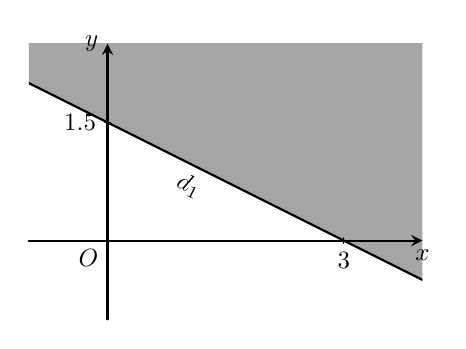
\begin{tikzpicture}[line join=round, line cap=round,>=stealth,thick]
			\tikzset{every node/.style={scale=0.9}}
			\begin{scope}
				\clip (-1,-1) rectangle (4,2.5);
				\fill[black!35] (-3,3)--(6,3)--(6,-1.5)--cycle;
				\draw (-2,2.5)--(5,-1) node [pos=0.45, below, sloped] {$d_1$};
			\end{scope}
			\draw[->] (-1,0)--(4,0) node[below]{$x$};
			\draw[->] (0,-1)--(0,2.5) node[left]{$y$};
			\draw (0,0) node[below left]{$O$};
			\foreach \x in {3}
			\draw[thin] (\x,1pt)--(\x,-1pt) node [below] {$\x$};
			\foreach \y in {1.5}
			\draw[thin] (1pt,\y)--(-1pt,\y) node [left] {$\y$};
		\end{tikzpicture}
		}
		\item $3x-4y\geq -3$.
		\immini{
		Vẽ đường thẳng $d_2\colon 3x-4y=-3 $.\\
		Lấy điểm $O(0;0)$. Ta có $3\cdot 0-4\cdot 0=0>-3$.\\
		Vậy miền nghiệm của bất phương trình $3x-4y\geq -3$ là nửa mặt phẳng không bị gạch chứa điểm $O(0;0)$ kể cả đường thẳng $d_2$.
		}
		{
		\begin{tikzpicture}[line join=round, line cap=round,>=stealth,thick]
			\tikzset{label style/.style={font=\footnotesize}}
			\begin{scope}
				\clip (-2,-3) rectangle (2,3);
				\fill[pattern=north west lines] (-6,-3.75)--(-6,3.75)--(4,3.75)--cycle;
				\draw (3,3)--(-5,-3) node [pos=0.45, above, sloped] {$d_2$};
			\end{scope}
			\draw[->] (-2,0)--(2,0) node[below]{$x$};
			\draw[->] (0,-1.5)--(0,3) node[left]{$y$};
			\draw (0,0) node[below left]{$O$};
			\foreach \x in {-1,1}
			\draw[thin] (\x,1pt)--(\x,-1pt) node [below] {$\x$};
			\foreach \y in {-1,1}
			\draw[thin] (1pt,\y)--(-1pt,\y) node [left] {$\y$};
		\end{tikzpicture}
		}
		\item $y\geq -2x+4$.
		\immini{
		Bất phương trình đã cho viết lại thành: $2x+y\ge 4$.\\
		Vẽ đường thẳng $d_3\colon 2x+y=4$.\\
		Lấy điểm $O(0;0)$. Ta có $2\cdot 0+0=0<4$.\\
		Vậy miền nghiệm của bất phương trình $2x+y\ge 4$ là nửa mặt phẳng không bị gạch không chứa điểm $O(0;0)$ kể cả đường thẳng $d_3$.
		}
		{
		\begin{tikzpicture}[line join=round, line cap=round,>=stealth,thick]
			\tikzset{label style/.style={font=\footnotesize}}
			\begin{scope}
				\clip (-1.5,-1.5) rectangle (2.5,4.5);
				\fill[pattern=north west lines] (-3,10)--(-3,-4)--(4,-4)--cycle;
				\draw (-1,6)--(3.5,-3) node [pos=0.45, above, sloped] {$d_3$};
			\end{scope}
			\draw[->] (-1.5,0)--(3,0) node[below]{$x$};
			\draw[->] (0,-1.5)--(0,5) node[left]{$y$};
			\draw (0,0) node[below left]{$O$};
			\foreach \x in {-1,1,2}
			\draw[thin] (\x,1pt)--(\x,-1pt) node [below] {$\x$};
			\foreach \y in {-1,1,2,3,4}
			\draw[thin] (1pt,\y)--(-1pt,\y) node [left] {$\y$};
		\end{tikzpicture}
		}
		\item $y<1-2x$.
		\immini{
		Bất phương trình đã cho viết lại thành: $2x+y<1$.\\
		Vẽ đường thẳng $d_4\colon 2x+y=1$.\\
		Lấy điểm $O(0;0)$. Ta có $2\cdot 0+0=0<1$.\\
		Vậy miền nghiệm của bất phương trình $2x+y<1$ là nửa mặt phẳng không bị gạch chứa điểm $O(0;0)$ không kể đường thẳng $d_4$.
		}
		{
		\begin{tikzpicture}[line join=round, line cap=round,>=stealth,thick]
			\tikzset{label style/.style={font=\footnotesize}}
			\begin{scope}
				\clip (-2,-3) rectangle (2,3);
				\fill[pattern=north west lines] (-3,7)--(3,7)--(3,-5)--cycle;
				\draw (-1,3)--(2,-3) node [pos=0.45, above, sloped] {$d_4$};
			\end{scope}
			\draw[->] (-1.5,0)--(2,0) node[below]{$x$};
			\draw[->] (0,-3)--(0,3) node[left]{$y$};
			\draw (0,0) node[below left]{$O$};
			\foreach \x in {-1,1}
			\draw[thin] (\x,1pt)--(\x,-1pt) node [below] {$\x$};
			\foreach \y in {-1,1}
			\draw[thin] (1pt,\y)--(-1pt,\y) node [left] {$\y$};
		\end{tikzpicture}
		}
	\end{enumerate}
	}
\end{bt}
\begin{bt}%[0D2H1-2]
	Phần không gạch (không kể $d$) ở mỗi Hình $a$, Hình $b$, Hình $c$ là miền nghiệm của bất phương trình nào?
	\begin{center}
		\begin{tikzpicture}[line join=round, line cap=round,>=stealth,thick,scale=.8]
			\tikzset{label style/.style={font=\footnotesize}}
			\begin{scope}
				\clip (-1,-3) rectangle (2.5,2);
				\fill[pattern=north west lines] (-3,-5)--(-3,4)--(6,4)--cycle;
				\draw (-1,-3)--(4,2) node [pos=0.45, below, sloped] {$d$};
			\end{scope}
			\draw[->] (-1,0)--(2.5,0) node[below]{$x$};
			\draw[->] (0,-3)--(0,2) node[left]{$y$};
			\draw (0,0) node[below left]{$O$};
			\foreach \x in {1,2}
			\draw[thin] (\x,1pt)--(\x,-1pt) node [below] {$\x$};
			\foreach \y in {-2,1}
			\draw[thin] (1pt,\y)--(-1pt,\y) node [left] {$\y$};
			\node[below] at (current bounding box.south){\it Hình $a$};
		\end{tikzpicture}
		\begin{tikzpicture}[line join=round, line cap=round,>=stealth,thick,scale=.8]
			\tikzset{label style/.style={font=\footnotesize}}
			\begin{scope}
				\clip (-1.5,-1.5) rectangle (4,5);
				\fill[pattern=north west lines] (-9,5.5)--(-9,-3.5)--(9,-3.5)--cycle;
				\draw (-8,5)--(8,-3) node [pos=0.45, above, sloped] {$d$};
			\end{scope}
			\draw[->] (-1.5,0)--(4,0) node[below]{$x$};
			\draw[->] (0,-1.5)--(0,2) node[left]{$y$};
			\draw (0,0) node[below left]{$O$};
			\foreach \x in {1,2}
			\draw[thin] (\x,1pt)--(\x,-1pt) node [below] {$\x$};
			\foreach \y in {1}
			\draw[thin] (1pt,\y)--(-1pt,\y) node [left] {$\y$};
			\node[below] at (current bounding box.south){\it Hình $b$};
		\end{tikzpicture}
		\begin{tikzpicture}[line join=round, line cap=round,>=stealth,thick,scale=.8]
			\tikzset{label style/.style={font=\footnotesize}}
			\begin{scope}
				\clip (-1.5,-2) rectangle (3,3);
				\fill[pattern=north west lines] (-4,-4)--(5,-4)--(5,5)--cycle;
				\draw (3,3)--(-3,-3) node [pos=0.45, above, sloped] {$d$};
			\end{scope}
			\draw[->] (-1.5,0)--(3,0) node[below]{$x$};
			\draw[->] (0,-2)--(0,2) node[left]{$y$};
			\draw (0,0) node[below right]{$O$};
			\foreach \x in {1}
			\draw[thin] (\x,1pt)--(\x,-1pt) node [below] {$\x$};
			\foreach \y in {1}
			\draw[thin] (1pt,\y)--(-1pt,\y) node [left] {$\y$};
			\draw[dashed] (1,0)--(1,1)node[above]{$ M $}--(0,1);
			\node[below] at (current bounding box.south){\it Hình $c$};
		\end{tikzpicture}
	\end{center}
\loigiai{
	\begin{enumerate}
		\item Xét Hình $a$.\\
		Ta có $d$ qua hai điểm $(2;0)$ và $(0;-2)$ nên phương trình của $d$ là $y=x-2$.\\
		Xét $y<x-2 $.\\
		Lấy điểm $O(0;0)$ ta có $0<0-2$ sai suy ra miền chứa điểm $O(0;0)$ không là miền nghiệm của bất phương trình $y<x-2$.\\
		Vậy phần không gạch (không kể $d$) là miền nghiệm của bất phương trình $y<x-2$.
		\item Xét Hình $b$.\\
		Ta có $d$ qua hai điểm $(2;0)$ và $(0;1)$ nên phương trình của $d$ là $y=-\dfrac{1}{2}x+1$.\\
		Xét $y<-\dfrac{1}{2}x+1$.
		Lấy điểm $O(0;0)$ ta có $0<-\dfrac{1}{2}\cdot 0+1$ đúng suy ra miền chứa điểm $O(0;0)$ là miền nghiệm của bất phương trình $y<-\dfrac{1}{2}x+1$.\\
		Vậy phần không gạch (không kể $d$) là miền nghiệm của bất phương trình \break$y>-\dfrac{1}{2}x+1$.
		\item Xét Hình $c$.\\
		Ta có $d$ qua hai điểm $(0;0)$ và $(1;1)$ nên phương trình của $d$ là $y=x$.\\
		Xét $y<x$.
		Lấy điểm $I(0;1)$ ta có $1<0$ sai suy ra miền chứa điểm $I(0;1)$ không là miền nghiệm của bất phương trình $y<x$.\\
		Vậy phần không gạch (không kể $d$) là miền nghiệm của bất phương trình \break$y>x$.
	\end{enumerate}
	}
\end{bt}
\begin{bt}%[0D2H1-3]
	Một gian hàng trưng bày bàn và ghế rộng $60$ m$^2$. Diện tích để kê một chiếc ghế là $0{,}5$ m$^2$, một chiếc bàn là $1{,}2$ m$^2 $. Gọi $x$ là số chiếc ghế, $y$ là số chiếc bàn được kê ($x$, $y\in\mathbb N$). Viết bất phương trình bậc nhất hai ẩn $x$, $y$ cho phần mặt sàn để kê bàn và ghế, biết diện tích mặt sàn dành cho lưu thông tối thiểu là $12$ m$^2$.
\loigiai{
	Diện tích kê $x$ chiếc ghế là $0{,}5x$ m$^2$.\\
	Diện tích kê $ y $ chiếc bàn là $1{,}2y$ m$^2$.\\
	Theo đề bài ta có $0{,}5x+1{,}2y\leq 60-12\Leftrightarrow 0{,}5x+1{,}2y\leq 48\Leftrightarrow 5x+12y\leq 480$.
	}
\end{bt}
\begin{bt}%[0D2V1-3]
	Bạn An giải $10$ bài Toán trong $20$ phút thì đúng được $80\%$ số bài Toán, giải $12$ bài Lý trong $15$ phút thì đúng được $\dfrac{3}{4}$ số bài Lý. Viết bất phương trình bậc nhất hai ẩn cho thời gian giải $x$ bài Toán đúng và $y$ bài Lý đúng, biết thời gian giải ít hơn $150$ phút ($x$, $y\in\mathbb N$).
\loigiai{
	Sau $20$ phút An làm đúng được $10\cdot 80\%=8$ bài Toán.\\
	Suy ra thời gian An giải đúng $x$ bài Toán là $\dfrac{20x}{8}=\dfrac{5x}{2}$ phút.\\
	Sau $15$ phút An làm đúng được $12\cdot \dfrac{3}{4}=9$ bài Lý.\\
	Suy ra thời gian An giải đúng $y$ bài Lý là $\dfrac{15y}{9}=\dfrac{5y}{3}$ phút.\\
	Vì thời gian giải ít hơn $150$ phút nên ta có
	\[\dfrac{5x}{2}+\dfrac{5x}{3}<150\Leftrightarrow 3x+2y<180.\]
	}
\end{bt}
\begin{bt}%[0D2H1-3]%
	Một công ty sản xuất hai loại sản phẩm gồm sản phẩm $X$ và sản phẩm $Y$. Chi phí sản xuất một sản phẩm $X$ là $2$ triệu đồng, sản xuất một sản phẩm $Y$ là $3$ triệu đồng. Chi phí thuê mặt bằng kho chứa là $100$ triệu đồng.
	\begin{enumerate}
		\item Tính tổng chi phí công ty sản xuất $200$ sản phẩm loại $X$ và $150$ sản phẩm loại $Y$.
		\item Gọi $x$  và $y$  lần lượt là số sản phẩm $X$ và sản phẩm $Y$ công ty sản xuất. Biết vốn sản xuất của công ty là $1$ tỉ đồng. Viết bất phương trình biểu thị mối liên hệ giữa $x$  và $y$.
	\end{enumerate}
\loigiai{
	\begin{enumerate}
		\item Tổng chi phí công ty sản xuất $200$ sản phẩm loại $X$ và $150$ sản phẩm loại $Y$ là
		$$200\cdot2+150\cdot3+100=950 \, \text{triệu đồng.}$$
		\item Chi phí sản xuất $x$ sản phẩm $X$ là $2x$ triệu đồng.\\
		Chi phí sản xuất $y$ sản phẩm $Y$ là $3x$ triệu đồng.\\
		Chi phí thuê mặt bằng kho chứa là $100$ triệu đồng.\\
		Tổng chi phí là $2x+3y+100$ triệu đồng.\\
		Vì  vốn sản xuất của công ty là $1$ tỉ đồng $=$ $1\,000$ triệu đồng.\\
		Do đó bất phương trình  biểu thị mối liên hệ giữa $x$  và $y$ là
		$$2x+ 3y +100\le 1\,000\Leftrightarrow 2x+3y\le 900.$$
		Vậy bất phương trình cần tìm là $2x+3y\le 900$.
	\end{enumerate}
	}
\end{bt}
\begin{bt}%[0D2V1-3]
	Nhân ngày Nhà giáo Việt Nam $20/11$, Công viên nước Đầm Sen và Công đoàn ngành giáo dục Thành phố Hồ Chí Minh tổ chức hội thi đua thuyền rồng dành cho giáo viên của tất cả các trường THPT trên địa bàn và được tổ chức tại Đầm Sen. Vé vào cổng được bán ra cho giáo viên và học sinh có hai loại:
	\begin{itemize}
		\item Loại 1 (dành cho học sinh): $20\,000$ đồng/vé;
		\item Loại 2 (dành cho giáo viên): $30\,000$ đồng/vé.
	\end{itemize}
	Công ty công viên nước Đầm Sen tính toán rằng, để không phải bù lỗ thì số tiền vé thu được khi vào cổng này phải đạt tối thiểu $30$ triệu đồng.\\
	Hỏi số lượng vé bán được trong những trường hợp nào thì công viên nước Đầm Sen phải bù lỗ?
\loigiai{
	Gọi $x$ là số lượng vé loại $1$ bán được $(x \in \mathbb{N})$. \\
	Gọi $y$ là số lượng vé loại $2$ bán được $(y \in \mathbb{N})$. \\
	Số tiền bán vé thu được là $20x+30y$ (nghìn đồng).\\
	Người ta sẽ phải bù lỗ trong trường hợp số tiền bán vé nhỏ hơn $30$ triệu đồng, tức là $20x+30y<30\,000$ hay $2x+3y<3000$.\\
	Như vậy việc giải quyết bài toán dẫn đến việc đi tìm miền nghiệm của bất phương trình $2x+3y<3000$.
	\immini{
	Miền nghiệm của bất phương trình bậc nhất hai ẩn này được xác định như sau
	\begin{itemize}
		\item Vẽ đường thẳng $d\colon 2x+3y=3000$ trên mặt phẳng toạ độ $Oxy$.
		\item Ta lấy gốc toạ độ $O(0;0)$ không thuộc $d$ và thay $x=0, y=0$ vào biểu thức $2x+3y$ ta được $2 \cdot 0 + 3 \cdot 0 =0<3000$.
	\end{itemize}
	Do đó miền nghiệm của bất phương trình là nửa mặt phẳng bờ $d$ chứa gốc toạ độ không kể đường thẳng $d$.
	}{
	\begin{tikzpicture}[line join=round, line cap=round,>=stealth,thick]
		\tikzset{label style/.style={font=\footnotesize}}
		\begin{scope}
			\clip (-1,3) rectangle (4.5,-1.3);
			\fill[pattern=north west lines,opacity=0.4] (-1.5,3)--(6,3)--(6,-2)--cycle;
			\draw[dashed] (0,1)--(1.5,1)--(1.5,0);
			\draw [thick,dashed](-1.5,3)--(6,-2) node [pos=0.75, below, sloped] {$(d)$};
		\end{scope}
		\draw[->] (-1,0)--(4.6,0) node[below]{$x$};
		\draw[->] (0,-1)--(0,3.1) node[left]{$y$};
		\draw (0,0) node[below left]{$O$};
		\foreach \x in {2,3}
		\draw[thin] (\x,1pt)--(\x,-1pt);
		\foreach \y in {1,2}
		\draw[thin] (1pt,\y)--(-1pt,\y);
		\fill[red] (1.5,1) circle (1pt);
		\fill (0,2) circle (1pt) node [above right] {$A$};
		\fill (3,0) circle (1pt) node [above right] {$B$};
		\draw (0,2) node [left] {$1000$}
		(0,1) node [left] {$500$}
		(1.5,0) node [below] {$750$}
		(3,0) node [below] {$1500$};
	\end{tikzpicture}
	}
	Vậy nếu bán được số vé loại $1$ là $x$ và số vé loại $2$ là $y$ mà điểm $(x; y)$ nằm trong miền tam giác $OAB$ không kể cạnh $AB$ thì công viên nước Đầm Sen sẽ phải bù lỗ.\\
	Nếu điểm $(x; y)$ nằm trên đoạn thẳng $AB$ thì công viên nước Đầm Sen hoà vốn.
	}
\end{bt}


\baitaptn
%-------------Trắc nghiệm nhiều lựa chọn
\ind{PHẦN I.} \inden{Câu trắc nghiệm nhiều phương án lựa chọn. Mỗi câu hỏi học sinh chỉ chọn một phương án.}
\setcounter{ex}{0}
\Opensolutionfile{ans}[ans/ansC2B3-nlc]
%%%==============Câu_1============%%%
\begin{ex}%[0D2N1-1]%
	Trong các bất phương trình sau, bất phương trình nào là bất phương trình bậc nhất hai ẩn?
	\choice
	{$2x-5y+3z \leq 0$}
	{$3x^2+2x-4> 0$}
	{$2x^2+5y > 3$}
	{\True $2x+3y < 5$}
\loigiai{
	Bất phương trình $2x+3y < 5$ là bất phương trình bậc nhất hai ẩn.
	}
\end{ex}
%%%==============Câu_2============%%%
\begin{ex}%[0D2N1-1]%
	Bất phương trình nào dưới đây \textbf{không} phải là bất phương trình bậc nhất $2$ ẩn?
	\choice
	{ $x+y-2 \geq 0$}
	{\True $2x+y-xy+2 \leq 0$}
	{$x+0y \leq 0$}
	{ $x-y-2 \geq 0$}
\loigiai{
	Bất phương trình $2x+y-xy+2 \leq 0$ không phải là bất phương trình bậc nhất $2$ ẩn.
	}
\end{ex}
%%%==============Câu_3============%%%
\begin{ex}%[0D2N1-1]%
	Cặp số nào sau đây là nghiệm của bất phương trình $-2(x-y)+y>3$?
	\choice
	{\True $(-4 ; 4)$}
	{$(4 ;-4)$}
	{$(-1 ;-2)$}
	{$(2 ; 1)$}
\loigiai{
	Thay $x=-4$; $y=4$ và  $-2(x-y)+y>3$ ta được $20>3$ (đúng) nên $(-4 ; 4)$ là nghiệm.
	}
\end{ex}
%%%==============Câu_4============%%%
\begin{ex}%[0D2N1-2]%
	Điểm $A(5 ;-3)$ là điểm thuộc miền nghiệm của bất phương trình nào sau đây?
	\choice
	{\True $5x-2y+1 \geq 0$}
	{$x-2y<0$}
	{$-3x+y+2>0$}
	{$2x-3y \leq 0$}
\loigiai{
	Thay $x=5$ và $y=-3$ vào từng bất phương trình:
	\begin{itemize}
		\item $5 \cdot 5 - 2 \cdot (-3) + 1 = 25 + 6 + 1 = 32 \geq 0$ (thỏa mãn)
		\item $5 - 2 \cdot (-3) = 5 + 6 = 11 > 0$ (không thỏa mãn)
		\item $-3 \cdot 5 + (-3) + 2 = -15 - 3 + 2 = -16 < 0$ (không thỏa mãn)
		\item $2 \cdot 5 - 3 \cdot (-3) = 10 + 9 = 19 \leq 0$ (không thỏa mãn)
	\end{itemize}
	Kết quả là $5x-2y+1 \geq 0$.
	}
\end{ex}
%%%==============Câu_5============%%%
\begin{ex}%[0D2N1-2]%
	Miền nghiệm của bất phương trình $3 x-y>3$ được xác định bởi nửa mặt phẳng (phần \textbf{không} bị gạch, không kể $d$ ) nào sau đây?
	\choice
	{\begin{tikzpicture}[scale=1, font=\footnotesize, line join=round, line cap=round, >=stealth]
	\draw[->]({-1},0)--({4},0)node[right]{$x$};
	\draw[->](0,{-2})--(0,{2})node[above]{$y$};
	\draw(0,0) node[below left]{$O$};
	\clip ({-1+0.1},{-2+0.1}) rectangle ({4-0.1},{2-0.1});
	\path [pattern=north east lines,pattern color = black,opacity=0.8] ({-1},{2})--plot[domain={-1}:{4}] (\x,{1/3*\x+-1})--({4},{2})--cycle;
	\draw plot[domain={-1}:{4}] (\x,{1/3*\x+-1});
	\draw[fill=black]
	(3,0) circle (0.04) node[below]{$3$}
	(0,-1) circle (0.04) node[below right]{$-1$}
	;
	\end{tikzpicture}}
	{\True \begin{tikzpicture}[scale=1, font=\footnotesize, line join=round, line cap=round, >=stealth]
	\draw[->]({-1},0)--({3},0)node[right]{$x$};
	\draw[->](0,{-4})--(0,{1})node[above]{$y$};
	\draw(0,0) node[below left]{$0$};
	\clip ({-1+0.1},{-4+0.1}) rectangle ({3-0.1},{1-0.1});
	\path [pattern=north east lines,pattern color = black,opacity=0.8] ({-1},{1})--plot[domain={-1}:{3}] (\x,{3*\x+-3})--({3},{1})--cycle;
	\draw plot[domain={-1}:{3}] (\x,{3*\x+-3});
	\draw[fill=black]
	(1,0) circle (0.04) node[below right]{$1$}
	(0,-3) circle (0.04) node[right]{$-3$}
	;
	\end{tikzpicture}}
	{\begin{tikzpicture}[scale=1, font=\footnotesize, line join=round, line cap=round, >=stealth]
	\draw[->]({-1},0)--({3},0)node[right]{$x$};
	\draw[->](0,{-4})--(0,{1})node[above]{$y$};
	\draw(0,0) node[below left]{$0$};
	\clip ({-1+0.1},{-4+0.1}) rectangle ({3-0.1},{1-0.1});
	\path [pattern=north east lines,pattern color = black,opacity=0.8] ({-1},{-4})--plot[domain={-1}:{3}] (\x,{3*\x+-3})--({3},{-4})--cycle;
	\draw plot[domain={-1}:{3}] (\x,{3*\x+-3});
	\draw[fill=black]
	(1,0) circle (0.04) node[above left]{$1$}
	(0,-3) circle (0.04) node[left]{$-3$}
	;
	\end{tikzpicture}}
	{\begin{tikzpicture}[scale=1, font=\footnotesize, line join=round, line cap=round, >=stealth]
	\draw[->]({-1},0)--({4},0)node[right]{$x$};
	\draw[->](0,{-2})--(0,{2})node[above]{$y$};
	\draw(0,0) node[below left]{$0$};
	\clip ({-1+0.1},{-2+0.1}) rectangle ({4-0.1},{1-0.1});
	\path [pattern=north east lines,pattern color = black,opacity=0.8] ({-1},{-2})--plot[domain={-1}:{4}] (\x,{1/3*\x+-1})--({4},{-2})--cycle;
	\draw plot[domain={-1}:{4}] (\x,{1/3*\x+-1});
	\draw[fill=black]
	(3,0) circle (0.04) node[above]{$3$}
	(0,-1) circle (0.04) node[above left]{$-1$}
	;
	\end{tikzpicture}}
	\loigiai
	{
	Miền nghiệm của $3x-y>3$ là nửa mặt phẳng bờ là đường thẳng $3x-y=3$ đi qua hai điểm $(1;0)$ và $(0;-3)$ và không chứa điểm $(0;0)$ không kể cả bờ.
	}
\end{ex}
%%%==============Câu_6============%%%
\begin{ex}%[0D2N1-2]%
	\immini[thm]{Bất phương trình bậc nhất hai ẩn nào có miền nghiệm như hình vẽ dưới đây (phần không tô đậm, kể cả đường thẳng)?
	\choice
	{$3x + 2y < 300$}
	{\True $3x + 2y \geq 300$}
	{$3x + 2y > 300$}
	{$3x + 2y \leq 300$}}
	{\begin{tikzpicture}[>=stealth,line join=round,line cap=round,font=\footnotesize,scale=0.8]
			\draw[->,line width = 1pt] (-1.5,0)--(0,0) node[below left]{$O$}--(3.5,0) node[below]{$x$};
			\draw[->,line width = 1pt] (0,-1.8) --(0,4.4) node[right]{$y$};
			\fill (-1.2,0) node[below]{$-50$};
			\fill (-1,0) circle (1pt);
			\fill (1,0) node[below]{$50$} circle (1pt);
			\fill (2,0) node[above right]{$100$} circle (1pt);
			\fill (0,-1) node[left]{$-50$} circle (1pt);
			\fill (0,1) node[left]{$50$} circle (1pt);
			\fill (0,3) node[left]{$150$} circle (1pt);
			\clip (-1.5,-1.8) rectangle (3.5,4.4);
			\draw [thick, domain=-1.5:3.2, samples=100] %d1
			plot (\x, {-1.5*(\x) + 3});			
			\fill[opacity=.2,pattern= north east lines] (-1.5,5.25)--(4.5,5.25)--(4.5,-1.8)--(3.2,-1.8)--cycle;
		\end{tikzpicture}}	
\loigiai{
	Xét $O(0;0) \notin (d)\colon 3x + 2y = 300$.\\
	Ta có $3\cdot 0 + 2\cdot 0 = 0 < 300$ nên bất phương trình bậc nhất hai ẩn $3x + 2y \geq 300$ có miền nghiệm như hình vẽ trên.
	}
\end{ex}
%%%============Câu_7==============%%%
\begin{ex}%[0D2H1-2]
	\immini[thm]
	{Nửa mặt phẳng không bị gạch (không kể $d$) ở hình bên là miền nghiệm của bất phương trình nào sau đây?
	\choice
	{$3x+y<3$}
	{$x+3y>3$}
	{$x+3y<3$}
	{\True $3x+y>3$}}
	{\begin{tikzpicture}[line cap=round,line join=round,font=\footnotesize,>=stealth,scale=0.75]
	\draw[->] (-2,0)--(2,0) node[below] {$x$};
	\draw[->] (0,-1)--(0,4) node[right] {$y$};
	\fill (0,0) circle (1pt) node [below left] {$O$};
	\draw [samples=100, domain=-1/3:4/3] plot (\x, {-3*(\x)+3});
	\fill [pattern=north west lines] (-2,4)--plot[domain=-1/3:4/3] (\x, {-3*(\x)+3})--(-2,-1)--(-2,4);
	\fill (1,0) node[shift={(80:1.5ex)}]{$1$} circle(1pt)
	(0,3) node[shift={(0:1ex)}]{$3$} circle(1pt)
	(-1/3,4) node[shift={(90:1ex)}]{$d$} circle(0pt)
	;
	\end{tikzpicture}}
\loigiai{
	Ta có đường thẳng $d$ qua $(1;0)$ và $(0;3)$ nên $d$ có phương trình $d\colon 3x+y=3$.\\
	Mặt khác, $3\cdot0+0=0<3$ nên miền nghiệm trong hình vẽ là nghiệm của bất phương trình $3x+y<3$ (chứa điểm $(0;0)$.).
	}
\end{ex}
%%%==============Câu_8============%%%
\begin{ex}%[0D2H1-2]%
	\immini[thm]{
	Miền\textbf{ không} tô đậm là miền nghiệm của bất phương trình nào sau đây?
	\choice
	{\True $x+y-4>0$}
	{$x-y+4<0$}
	{$x-y-4>0$}
	{$x+y-4<0$}
	}
	{
	\begin{tikzpicture}[line join=round, line cap=round,>=stealth,thick,scale=0.5]
		\tikzset{every node/.style={scale=0.9}}
		\begin{scope}
			\clip (-1,-1) rectangle (5,5);
			\fill[pattern=north east lines] (-2,6)--(-2,-2)--(6,-2)--cycle;
			\draw (-1,5)--(5,-1);
		\end{scope}
		\draw[->] (-1,0)--(5,0) node[below]{$x$};
		\draw[->] (0,-1)--(0,5) node[left]{$y$};
		\draw (0,0) node[below left]{$O$};
		\foreach \x in {4}
		\draw[thin] (\x,1pt)--(\x,-1pt) node [above] {$\x$};
		\foreach \y in {4}
		\draw[thin] (1pt,\y)--(-1pt,\y) node [right] {$\y$};
	\end{tikzpicture}
	}
	\loigiai
	{
	Đường thẳng $d$ đi qua điểm $(4;0)$ và $(0;4)$ có phương trình $x+y-4=0$.\\
	Gốc tọa độ không là nghiệm của bất phương trình nên miền không tô đậm là miền nghiệm của bất phương trình $x+y-4>0$.
	}
\end{ex}
%%%==============Câu_9============%%%
\begin{ex}%[0D2H1-2]%
	Điểm $M(1;1)$ thuộc miền nghiệm của bất phương trình nào sau đây?
	\choice
	{\True $ x-2y <1$}
	{$x-y-1>0 $}
	{$x> y+5 $}
	{$ x+ y>2  $}
\loigiai{
	Thay $x=1$, $y=1$ vào bất phương trình $x-2y<1$ ta được $1-2<1 \Leftrightarrow -1<1$ (đúng).\\
	Suy ra $M(1;1)$ thuộc miền nghiệm của bất phương trình $x-2y<1$.}
\end{ex}
%%%==============Câu_10============%%%
\begin{ex}%[0D2H1-2]
	Cho đường thẳng $d\colon7x-9y+2=0$ chia mặt phẳng toạ độ làm hai nửa  mặt phẳng, trong đó miền nghiệm của bất phương trình $7x-9y+2>0$ là nửa mặt phẳng
	\choice
	{có bờ là đường thẳng $d$ và không chứa điểm $O(0;0)$}
	{\True không có bờ $d$ và chứa điểm $O(0;0)$}
	{có bờ là đường thẳng $d$ và chứa điểm $O(0;0)$}
	{không chứa bờ $d$ và không chứa điểm $O(0;0)$}
\loigiai{
	Ta có toạ độ điểm $O(0;0)$ thoả mãn bất phương trình $7x-9y+2>0$ nên miền nghiệm của bất phương trình $7x-9y+2>0$ là nửa mặt phẳng không có bờ $d$ và chứa điểm $O(0;0)$.
	}
\end{ex}
%%%==============Câu_11============%%%
\begin{ex}%%[0D2H1-3]
	Bạn Danh để dành được $900$ nghìn đồng. Trong một đợt ủng hộ trẻ em mồ côi, Danh đã lấy ra $x$ tờ tiền loại $50$ nghìn đồng, $y$ tờ tiền loại $100$ nghìn đồng để trao tặng. Một bất phương trình mô tả điều kiện ràng buộc đối với $x,y$ là
	\choice
	{\True $50x+100y \leq 900$}
	{$50x+100y \geq 900$}
	{$100x+50y \leq 900$}
	{$x+y=900$}
\loigiai{
	Bất phương trình mô tả điều kiện ràng buộc đối với $x,y$ là $50x+100y \leq 900$.
	}
\end{ex}
%%%==============Câu_12============%%%
\begin{ex}%[0D2H1-3]
	Cho bất phương trình $2x+3y-2<0$. Miền nghiệm của bất phương trình là
	\choice
	{\True nửa mặt phẳng chứa điểm $O$ có bờ là đường thẳng $2x+3y-2=0$ (không kể bờ)}
	{nửa mặt phẳng chứa điểm $O$ có bờ là đường thẳng $2x+3y-2=0$ (kể cả bờ)}
	{nửa mặt phẳng không chứa điểm $O$ có bờ là đường thẳng $2x+3y-2=0$ (không kể bờ)}
	{nửa mặt phẳng không chứa điểm $O$ có bờ là đường thẳng $2x+3y-2=0$ (kể cả bờ)}
\loigiai{
	\immini{Vẽ đường thẳng $2x+3y-2=0$.\\
	Xét điểm $O(0;0)$ không thuộc đường thẳng $2x+3y-2=0$.\\
	Ta có $P=2 \cdot 0+3 \cdot 0-2<0$.\\
	Vậy nửa mặt phẳng chứa điểm $O$ có bờ là đường thẳng $2x+3y-2=0$ (không kể bờ) là miền nghiệm của bất phương trình.}{
	\begin{tikzpicture}[scale=0.8, font=\footnotesize, line join=round, line cap=round, >=stealth]
		\clip(-2,-1) rectangle (3,2);
		\draw[line width=0.8pt,dash pattern=on 3pt off 3pt,fill=black,pattern=north east lines,pattern color=black](-4.08,3.38)--(-4.08,-7.81)--(4.74,-7.81)--(4.74,-2.49)--(-4.08,3.38);
		\draw [->,line width=0.4pt] (-2,0) -- (3,0);
		\draw [->,line width=0.4pt] (0,-1) -- (0,2);
		\begin{scriptsize}
			\draw (-0.3,1.8) node {$y$};
			\draw (2.95,-0.2) node {$x$};
			\draw (-0.3,-0.3) node {$O$};
			\draw [fill=black] (1,0) circle (1pt);
			\draw (1,0.25 ) node {$1$};
			\draw (0,1) node[right] {$2x+3y-2<0$};
		\end{scriptsize}
	\end{tikzpicture}}}
\end{ex}
\Closesolutionfile{ans}
\indapan{6}{ans/ansC2B3-nlc}
%---------------------Trắc nghiệm đúng sai
\ind{PHẦN II.} \inden{Câu trắc nghiệm đúng sai. Trong mỗi ý a), b), c), d) ở mỗi câu, học sinh chọn đúng hoặc sai.}
\setcounter{ex}{0}
\Opensolutionfile{ans}[ans/ansC2B3-ds]
%%%==============Câu_1============%%%
\begin{ex}%[0D2N1-1]
	Cho bất phương trình $2x-y<3$. \quad(1)
	\choiceTF
	{\True Cặp số $(1;1)$ là nghiệm của (1)}
	{  Cặp số $(2;0)$ là nghiệm của (1)}
	{  Cặp số $(0;-1)$ là nghiệm của (1)}
	{Cặp số $(5;8)$ là nghiệm của (1)}
\loigiai{
	\begin{itemchoice}
		\itemch Cặp số $(1;1)$ là nghiệm của (1).
		\itemch   Cặp số $(2;0)$ không là nghiệm của (1).
		\itemch Cặp số $(0;-1)$ là nghiệm của (1).
		\itemch Cặp số $(5;8)$ là nghiệm của (1).
	\end{itemchoice}
	}
\end{ex}
%%%==============Câu_2============%%%
\begin{ex}%[0D2H1-2]
	Cho bất phương trình $ax+by+4\ge 0$ có miền nghiệm là phần không tô đậm (kể cả biên là đường thẳng $d$) như hình sau
	\begin{center}
		\begin{tikzpicture}[scale=0.65, font=\footnotesize, line join=round, line cap=round, >=stealth]
			\draw[->] (-6,0)--(4,0) node[below] {$x$};
			\draw[->] (0,-1.5)--(0,5) node[left] {$y$};
			\draw(-6,-1)--(4,4);
			\draw (0,0) node[below left] {$O$};
			\fill[black] (-4,0) circle (1pt) node[below] {$-4$};
			\fill[black] (0,2) circle (1pt) node[right] {$2$};
			\fill[pattern=north east lines] (-6,-1)--(-6,5)--(4,5)--(4,4);
		\end{tikzpicture}
	\end{center}
	\choiceTF
	{ \True Điểm $O\left(0;0\right)$ thuộc miền nghiệm của bất phương trình $ax+by+4\ge 0$}
	{Đường thẳng $d: x+2y+4 =0 $ }
	{ \True $a+b=-1$}
	{Miền nghiệm của bất phương trình là nửa mặt phẳng có bờ là đường thẳng $d$ (kể cả $d$) và không chứa điểm $A\left(1;2\right)$}
\loigiai{
	\begin{itemchoice}
		\itemch
		Điểm $O$ thuộc miền nghiệm bất phương trình là đúng.
		\itemch
		Đường thẳng $ax+by+4 =0$ đi qua hai điểm $(-4;0)$ và $(0;2)$ nên  $\heva{& a = 1\\&  b = -2.}$\\
		Do đó $d\colon x-2y+4 =0$.
		\itemch
		Đường thẳng $d\colon x-2y+4 =0$ nên  $\heva{& a = 1\\&  b = -2}$. Suy ra $a+b=-1$.
		\itemch
		Với $a = 1$ và $b = -2$ thì bất phương trình là $x - 2y + 4 \ge 0$. \\
		Khi đó $1-2 \cdot 2+4\ge 0$ là đúng. Do đó, miền nghiệm của bất phương trình là nửa mặt phẳng có bờ là đường thẳng $d$ (kể cả $d$) và chứa điểm $A\left(1;2\right)$.
	\end{itemchoice}
	}
\end{ex}
%%%==============Câu_3============%%%
\newpage
\begin{ex}%[0D2H1-3]
	Một cửa hàng dành tối đa $10$ triệu đồng để nhập $x$ tạ gạo và $y$ tạ mì ($x, y\geq0$). Biết mỗi tạ gạo mua hết $1{,}5$ triệu đồng, mỗi tạ mì mua hết $1{,}2$ triệu đồng.
	\choiceTF
	{\True Số tiền dùng để mua $x$ tạ gạo và $y$ tạ mì là $1{,}5x + 1{,}2y$ (triệu)}
	{Bất phương trình biểu thị mối liên hệ giữa $x$ và $y$ là $1{,}5x+1{,}2y\ge10$}
	{\True $1{,}5x+1{,}2y\geq10$ là bất phương trình bậc nhất hai ẩn}
	{\True Miền nghiệm của bất phương trình $1{,}5x + 1{,}2y\leq10$ là nửa mặt phẳng bờ là đường thẳng $d\colon1{,}5x+1{,}2y=10$ chứa điểm $O(0;0)$}
\loigiai{
	\begin{itemchoice}
		\itemch
		Số tiền dùng để mua $x$ tạ gạo và $y$ tạ mì là $1{,}5x + 1{,}2y$ (triệu).
		\itemch
		Bất phương trình biểu thị mối liên hệ giữa $x$ và $y$ là $1{,}5x+1{,}2y\le10$.
		\itemch
		$1{,}5x+1{,}2y\geq 10$ là bất phương trình bậc nhất hai ẩn.
		\itemch
		Ta có $1{,}5\cdot0+ 1{,}2\cdot0\leq10$ đúng.\\
		Do đó miền nghiệm của bất phương trình $1{,}5x + 1{,}2y\leq10$ là nửa mặt phẳng bờ là đường thẳng $d\colon1{,}5x+1{,}2y=10$ chứa điểm $O(0;0)$.
	\end{itemchoice}
	}
\end{ex}
%%%==============Câu_4============%%%
\begin{ex}%[0D2V2-3]
	Một gia đình cần ít nhất $900$ đơn vị protein và $400$ đơn vị lipit trong thức ăn mỗi ngày. Mỗi kilôgam thịt bò chứa $800$ đơn vị protein và 200 đơn vị lipit. Mỗi kilôgam thịt lợn chứa $600$ đơn vị protein và $400$ đơn vị lipit. Biết rằng gia đình này chỉ mua nhiều nhất là $1{,}6$ kg thịt bò và $1{,}1$ kg thịt lợn; giá tiền 1 kg thịt bò là 250 nghìn đồng; 1 kg thịt lợn là 160 nghìn đồng. Giả sử gia đình đó mua $x$ kilôgam thịt bò và $y$ kilôgam thịt lợn.
	\choiceTF
	{\True Số protein chứa trong $x$ kilôgam thịt bò và $y$ kilôgam thịt lợn là $800 x+600 y$}
	{Bất phương trình biểu diễn số đơn vị lipit mà gia đình đó cần mỗi ngày là $2x+y \geq 2$}
	{\True Số tiền phải trả cho $x$ kilôgam thịt bò và $y$ kilôgam thịt lợn là $F(x ; y)=250 x+160 y$ (nghìn đồng)}
	{\True Mua $0{,}3$ kg thịt bò và $1{,}1$ thịt lợn thì chi phí ít nhất}
\loigiai{
	\begin{itemchoice}
		\itemch Mỗi kilôgam thịt bò chứa $800$ đơn vị protein và mỗi kilôgam thịt lợn chứa $600$ đơn vị protein. Nên Số protein chứa trong $x$ kilôgam thịt bò và $y$ kilôgam thịt lợn là
		$800 x+600 y.$
		\itemch Một gia đình cần ít nhất 400 đơn vị lipit trong thức ăn mỗi ngày nên ta có:
		$$
		200 x+400 y \geq 400 \Leftrightarrow x+2 y \geq 2.
		$$
		\itemch Vì số tiền mỗi kg thịt bò và thịt lợn lần lượt là $250$ nghìn đồng và $160$ nghìn đồng nên ta có $F(x ; y)=250 x+160 y$ (nghìn đồng).
		\itemch Gia đình này cần ít nhất $900$ đơn vị prô-tê-in và $400$ đơn vị li-pít trong thức ăn mỗi ngày nên ta có hệ bất phương trình sau:
		$$\heva{&800x+600y\geq 900\\&200x+400y\geq 400\\&0\leq x\leq 1{,}6\\&0\leq y\leq 1{,}1}\Leftrightarrow \heva{&8x+6y\geq 9\\&x+2y\geq 2\\&0\leq x\leq 1{,}6\\&0\leq y\leq 1{,}1.}$$
		\immini{Bài toán trở thành: Tìm GTNN của $F=45000x+35000y$ với $x$, $y$ thỏa hệ trên.\\
		Giải hệ bất phương trình trên, ta có miền nghiệm là tứ giác $ABCD$ (hình bên) với tọa độ các đỉnh là: $A(1{,}6;1{,}1)$, $B(1{,}6;0{,}2)$, $C(0{,}6;0{,}7)$, $D(0{,}3;1{,}1)$.\\
		Khi đó: \\Tại $A(1{,}6;1{,}1)$: $F=576$\\
		Tại $B(1{,}6;0{,}2)$: $F=432$\\
		Tại $C(0{,}6;0{,}7)$: $F=262$\\
		Tại $D(0{,}3;1{,}1)$: $F=251$.
		}
		{\begin{tikzpicture}[scale=1, font=\footnotesize, line join=round, line cap=round, >=stealth]
		\fill[pattern=north east lines] (-1,-1) -- (-1,2) -- (3,2) -- (3,-1) -- cycle;
		\fill[white] (1.6,1.1) -- (1.6,0.2) -- (0.6,0.7) --(0.3,1.1)-- cycle;
		\draw[->] (-1.3,0) -- (3.3,0)node[above]{$x$};
		\foreach \x in {1,2}
		\draw[shift={(\x,0)},color=black] (0pt,2pt) -- (0pt,-2pt) node[below left] {\footnotesize $\x$};
		\draw[->,color=black] (0,-1.2) -- (0,2.3)node[right]{$y$};
		\foreach \y in {1}
		\draw[shift={(0,\y)},color=black] (2pt,0pt) -- (-2pt,0pt) node[above right] {\footnotesize $\y$};
		\node[above left] at (0,0){$O$};
		\node[above left] at (1.6,1.1){$A$};
		\node[above right] at (1.6,0.2){$B$};
		\node[below left] at (0.6,0.7){$C$};
		\node[above right] at (0.3,1.1){$D$};
		\clip(-1,-1) rectangle (3,2);
		\draw[smooth,samples=100,domain=-1:3] plot(\x,{1.5-1.333333*(\x)});
		\draw[smooth,samples=100,domain=-1:3] plot(\x,{1-0.5*(\x)});
		\draw[,smooth,samples=100,domain=-1:3] plot(\x,{1.1-0*(\x)});
		\draw[smooth,samples=100,domain=-1:3] (1.6,-1)--(1.6,3);
		\end{tikzpicture}
		}
		Suy ra, $F$ nhỏ nhất khi $(x;y)=(0{,}3;1{,}1)$. Do đó gia đình này cần mua $0{,}3$ kg thịt bò và $1{,}1$ kg thịt lợn.
	\end{itemchoice}
	}
\end{ex}
\Closesolutionfile{ans}
\indapan{2}{ans/ansC2B3-ds}
\ind{PHẦN III.} \inden{Câu trả lời ngắn.}
\setcounter{ex}{0}
\Opensolutionfile{ans}[ans/ansC2B3-tln]
%-----Câu 1
\begin{ex}%[0D2H1-2]
	\immini{Nửa mặt phẳng không bị gạch (không kể $d$) ở hình bên là miền nghiệm của bất phương trình có dạng $ax+by-2>0$. Giá trị của $a+b$ bằng bao nhiêu?}
	{
	\begin{tikzpicture}[scale=1,line join=round, line cap=round,>=stealth]
		\tikzset{every node/.style={scale=0.9}}
		\begin{scope}
			\clip (-1,-2.5) rectangle (3.5,1.5);
			\fill[pattern=north west lines] (-2,-4)--(-2,2.5)--(4.5,2.5)--cycle;
			\draw (3.5,1.5)--(-0.5,-2.5);
		\end{scope}
		\draw[->] (-1,0)--(3.5,0) node[below]{$x$};
		\draw[->] (0,-2.5)--(0,1.7) node[left]{$y$};
		\draw (0,0) node[below left]{$O$};
		\foreach \x in {2,3}
		\draw[thin] (\x,1pt)--(\x,-1pt) node [above] {$\x$};
		\foreach \y in {-2,-1}
		\draw[thin] (1pt,\y)--(-1pt,\y) node [left] {$\y$};
		%	\draw[dashed,thin] (3,0)--(3,-1)--(0,-1);
	\end{tikzpicture}
	}
	\shortans{$0$}
\loigiai{
	Dựa vào hình ta thấy đường thẳng $d$ có hệ số góc khác $0$ nên gọi $(d)\colon y=ax+b$	.\\
	Ta có : $(2;0)\in (d)\Rightarrow 2a+b=0$ và $(0;-2)\in (d)\Rightarrow b=-2$,\\
	Vậy $(d)\colon y=x-2$ hay $x-y-2=0$.\\
	Mà $(0;0)$ không thuộc miền nghiệm $\Rightarrow x-y-2>0$.\\
	Do đó $a=1; b=-1 \Rightarrow a+b=0$.
	}
\end{ex}
\begin{ex}%[0D2V1-2]
	Cho bất phương trình $2x-(m+2)y+m\le 0$. Có bao nhiêu giá trị nguyên âm của tham số $m$ để bất phương trình có một nghiệm là $(1;3)$?
	\shortans{$2$}
\loigiai{
	Thay $(1;3)$ vào bất phương trình ta được  $2\cdot 1-(m+2)\cdot 3+m\le 0\Leftrightarrow m\ge -2$.\\
	Mà $m$ nguyên âm $\Rightarrow m=\left\lbrace -2;-1\right\rbrace$.\\
	Vậy có $2$ giá trị nguyên âm của tham số $m$ thỏa mãn bất phương trình đã cho.
	}
\end{ex}
\begin{ex}%[0D2H1-3]
	Bạn Lan mang $120\,000$ đồng đi nhà sách để mua một số quyển tập và bút. Biết rằng giá một quyển tập là $8\,000$ đồng và giá của một cây bút là $6\,000$ đồng. Bạn Lan có thể mua được $x$ quyển tập và $y$ cây bút. Bất phương trình theo $x$, $y$ diễn tả số quyển tập và cây bút mà bạn Lan mua là $4x+m y \leq n$. Tính $m+n$.
	\par\shortans{63}
\loigiai{
	Gọi $x$ là số quyển tập bạn Lan mua được, $y$ là số cây bút bạn Lan mua được. Khi đó \allowdisplaybreaks
	\begin{eqnarray*}
		8\,000x+6\,000y \le 120\,000 \Leftrightarrow 4x+3y\le 60.
	\end{eqnarray*}
	Khi đó, $m=3$ và $n=60$ nên $m+n=63$.
	}
\end{ex}
\begin{ex}%[0D2V1-3]
	Bạn Nam tiết kiệm được $450$ nghìn đồng. Trong đợt ủng hộ các bạn học sinh đồng bào miền Trung bị lũ lụt vừa qua, bạn Nam đã ủng hộ $x$ tờ tiền loại $20$ nghìn đồng, $y$ tờ tiền loại $10$ nghìn đồng. Khi đó bất phương trình biểu diễn tổng số tiền mà bạn Nam đã ủng hộ có dạng $mx+y\le n$. Tính giá trị của biểu thức $P=m+n$.
	\shortans{$47$}
\loigiai{
	Tổng số tiền bạn Nam đã ủng hộ là $20x + 10y$.\\
	Vì bạn Nam chỉ có tất cả $450$ nghìn đồng nên tổng số tiền bạn Nam đã ủng hộ không thể vượt quá $450$ nghìn đồng.\\
	Vậy ta có bất phương trình $20 x+10 y \leq 450\Leftrightarrow 2x+y\le 45$.\\
	Do đó  $m=2$, $n=45$. Suy ra $P=m+n=47$.
	}
\end{ex}
\begin{ex}%[0D2V1-3]
	Một đội sản xuất cần $3$ giờ để làm xong sản phẩm loại I và $2$ giờ để làm xong sản phẩm loại II. Biết thời gian tối đa cho việc sản xuất hai sản phẩm trên là $18$ giờ. Gọi $x$, $y$ lần lượt là số sản phẩm loại I, loại II mà đội làm được trong thời gian cho phép. Khi đó bất phương trình biểu diễn tổng thời gian làm xong hai loại sản phẩm trên có dạng $3x+by+c\le 0$. Tính giá trị của biểu thức $P=b+c$.
	\shortans{$-16$}
\loigiai{
	Tổng thời gian làm xong hai loại sản phẩm là $3x+ 2y$ giờ.\\
	Vì thời gian tối đa cho việc sản xuất hai sản phẩm trên là $18$ giờ,
	Vậy ta có bất phương trình $3x+2y \le 18\Leftrightarrow 3x+2y -18\le 0$.\\
	Do đó $b=2$, $c= -18$. Suy ra $P=b+c=-16$.
	}
\end{ex}
\begin{ex}%[0D2H1-3]
	Gia đình anh An muốn thuê một chiếc ô tô (có lái xe) trong một tuần. Giá thuê xe gồm 2 loại phí được cho như bảng sau
	\begin{center}
		\begin{tabular}{|c|c|c|}
			\hline
			& Phí cố định
			& Phí tính theo quảng đường
			di chuyến\\
			& (nghìn đồng/ngày)
			& (nghìn đồng/kilômét)\\
			\hline
			Tứ thứ Hai đến thứ Sáu & 600 & 7 \\
			\hline
			Thứ Bảy và Chủ nhật & 1400 & 14 \\
			\hline
		\end{tabular}
	\end{center}
	Gọi $x$ và $y$ lần lượt là số kilômét gia đình anh An đi trong các ngày từ thứ hai đến thứ sáu và trong hai ngày cuối tuần. Bất phương trình biểu thị mối liên hệ giữa $x$ và $y$ sao cho tổng số tiền anh An phải trả không quá $12$ triệu đồng có dạng $7x+my\le n$. Biểu thức $m+n$ có giá trị bằng
	\shortans[oly]{$6214$}
\loigiai{
	Phí thuê xe từ thứ hai đến thứ sáu là $7x+600\cdot5$ nghìn đồng.\\
	Phí thuê xe thứ bảy, chủ nhật là $14y+1400\cdot2$ nghìn đồng.\\
	Vì tổng số tiền phải trả không quá $12$ triệu đồng nên $$7x+600\cdot5+14y+1400\cdot2\le 12000 \Leftrightarrow7x+14y\le 6200.$$
	Vậy $m+n=6214$.
	}
\end{ex}
\Closesolutionfile{ans}
\indapan{3}{ans/ansC2B3-tln}
